\documentclass[a4paper,10pt]{article}
\usepackage[a4paper,bindingoffset=0.2in,%
left=1in,right=1in,top=1in,bottom=1in,%
footskip=.25in]{geometry}
\usepackage{graphicx}
\usepackage[utf8]{inputenc}
\usepackage{subcaption}
\title{Guide d'installation et d'utilisation du RCSF}
\author{Saad Errguibi - Audensiel Technologies}

\begin{document}

\maketitle
\section{Installation}
%\subsection{Les no \eu ds de capteurs}
Le montage sur la figure \ref{tx2} est à réaliser pour les 5 n\oe uds.
\begin{figure}[!h]
	\centering
	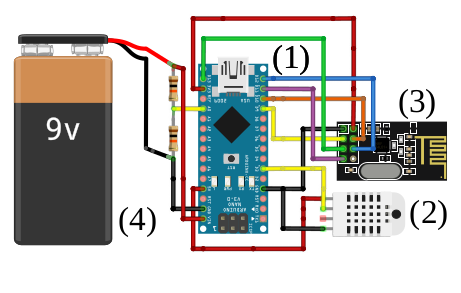
\includegraphics[scale=.8]{figures/tx2.pdf}
		\caption{Schéma de montage }
	\label{tx2}
\end{figure}
La connexion entre l'Arduino NANO V3 (ATmega 168) (\textit{cf}. figure \ref{fig1}) et la sonde de température (\textit{cf}. figure \ref{fig2}) est détaillée dans le tableau \ref{tab1}.
\begin{table}[!h]
	\centering
	\begin{tabular}{|c|c|c|c|c|}
		\hline 
		Pin DHT11 & $V_{cc}$ (1) & Data (2) & NC (3) & GND (4) \\ 
		\hline 
		Pin Arduino Nano & 5V & D2 &  & GND \\ 
		\hline 
	\end{tabular}
	\caption{Connexions entre le capteur et l'unité de traitement} \label{tab1} 	
\end{table}
\begin{figure}[h]
	\centering
	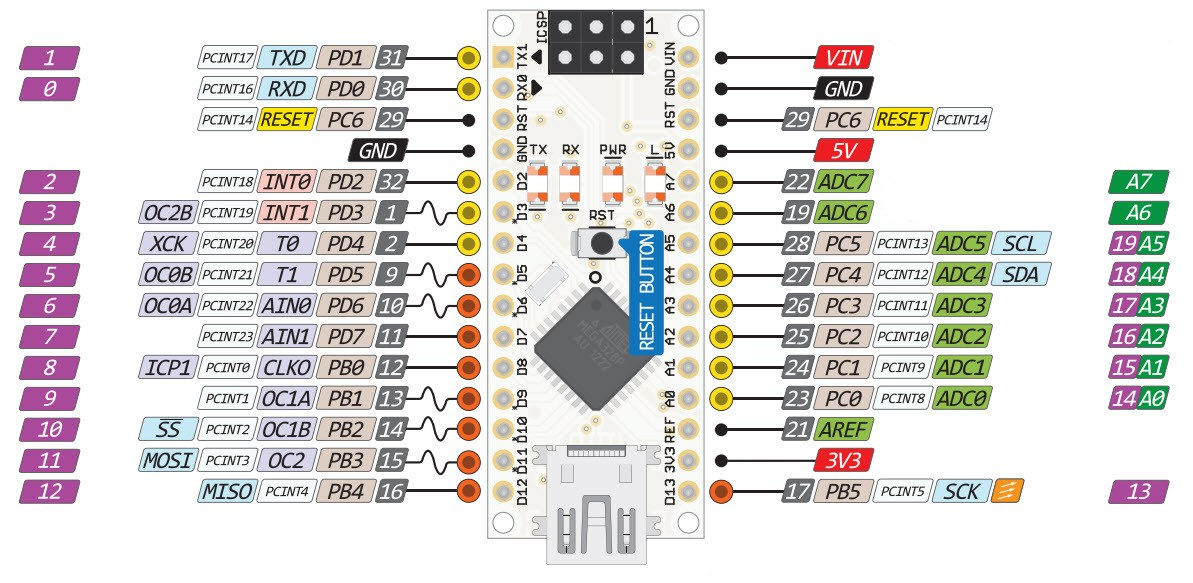
\includegraphics[scale=.5]{figures/nano.jpg}
		\caption{Arduino Nano V3 brochage}
		\label{fig1}
\end{figure}
\begin{figure}[h]
		\centering
	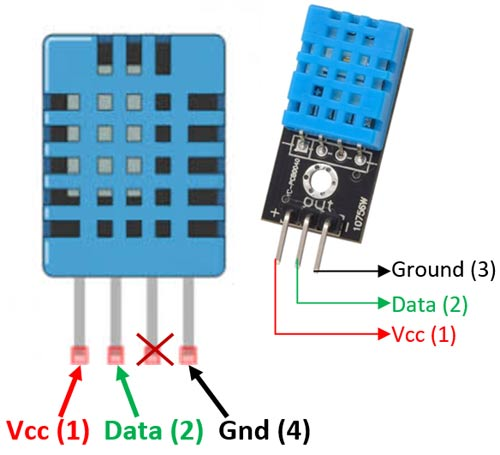
\includegraphics[scale=.49]{figures/dht.jpg}
		\caption{DHT11 brochage}
		\label{fig2}

%	\caption{Combined figure}
%	\label{fig:combined}
\end{figure}

La connexion entre l'Arduino NANO V3 (ATmega 168) (\textit{cf}. figure \ref{fig1}) et le module de communication nRF24L01 (\textit{cf}. figure \ref{fig2}) est détaillée dans le tableau \ref{tab2}.
\begin{table}[!h]
	\centering
	\begin{tabular}{|c|c|c|c|c|c|c|c|c|}
		\hline 
	nRF24L01 & GND (1) & VCC (2)& CE (3) & CSN (4) 	& SCK (5) 	& MOSI (6) 	& MISO (7) 	& IRQ (8) \\ 
		\hline 
	Arduino Nano & GND 	& 3.3 V	& D9 & D10	& D13 & D12	& D11 & NC\\ 
		\hline 
	\end{tabular}
	\caption{Connexions entre le le module de communication nRF24l01 et l'unité de traitement} \label{tab2} 	
\end{table}

Surveiller l'état de la batterie ce fait a l'aide de la broche analogique A0 de la carte Arduino. Le CAN de la carte Arduino accepte des tensions comprissent entre 0 et 5V. Un pont diviseur de tension avec deux résistances de 10 k$\Omega$ permet de réduire la tension d'alimentation de 9V à 4.5V ainsi l'état de la batterie des n \oe uds est surveiller. 

\subsection{Passerelle}
Le montage est à réaliser pour la passerelle.
\section{Utilisation}
Pour lancer les mesures, il faut se cordonnet a la passereselle (Raspberry Pi) en SSH.
puis lancer le script python gateway 



\medskip

%\bibliographystyle{unsrt}%Used BibTeX style is unsrt
%\bibliography{sample}

\end{document}
